\documentclass[aspectratio=169,10pt]{beamer}

\usetheme{default}
\usecolortheme{default}
\usepackage{amsmath,amssymb}
\usepackage{graphicx}
\usepackage{booktabs}
\usepackage{xcolor}
\usepackage{tikz}

% Shared result macros — auto-updated by update_report.py
% Main model (Stage 2, K=8, λ=0.1, 30 epochs)
\newcommand{\MAINPSNR}{34.66}
\newcommand{\MAINSSIM}{0.9959}
\newcommand{\MAINMSE}{0.0004}
\newcommand{\MAINEMSE}{0.0039}
\newcommand{\MAINDRIFTV}{0.01524}
\newcommand{\MAINDRIFTX}{0.02341}
\newcommand{\MAINDRIFTXX}{0.02748}
\newcommand{\MAINPSNRDIFF}{3.36}
% Ablation rows
\newcommand{\NOSTPSNR}{9.45}
\newcommand{\NOSTSSIM}{0.2112}
\newcommand{\NOSTDRIFTV}{0.51469}
\newcommand{\NOSTDRIFTX}{0.53594}
\newcommand{\LAMZPSNR}{34.58}
\newcommand{\LAMZSSIM}{0.9965}
\newcommand{\LAMZDRIFTV}{0.02507}
\newcommand{\LAMZDRIFTX}{0.02857}
\newcommand{\LAMONEPSNR}{32.23}
\newcommand{\LAMONESSIM}{0.9918}
\newcommand{\LAMINEPSNR}{34.52}
\newcommand{\LAMINESSIM}{0.9965}
\newcommand{\KTWOPSNR}{33.50}
\newcommand{\KTWOSSIM}{0.9946}
\newcommand{\KFOURPSNR}{33.94}
\newcommand{\KFOURSSIM}{0.9953}
\newcommand{\KSIXTEENPSNR}{34.34}
\newcommand{\KSIXTEENSSIM}{0.9960}
\newcommand{\DECPRTPSNR}{49.57}
\newcommand{\DECPRTSSIM}{0.9999}
% Stage 3: Planning evaluation (auto-filled by update_report.py)
\newcommand{\PLANVLMSR}{5\%}
\newcommand{\PLANVLMWMSR}{5\%}
\newcommand{\PLANBFSSR}{100\%}
\newcommand{\PLANVLMSTEPS}{14.0}
\newcommand{\PLANVLMWMSTEPS}{13.0}
\newcommand{\PLANBFSSTEPS}{14.0}


% ── Color palette ─────────────────────────────────────────────────────────────
\definecolor{ucsdblue}{RGB}{0,98,155}
\definecolor{ucsdgold}{RGB}{255,205,0}
\definecolor{softgray}{RGB}{245,245,247}
\definecolor{darkgray}{RGB}{60,60,60}
\definecolor{accentgreen}{RGB}{39,174,96}
\definecolor{accentred}{RGB}{192,57,43}

\setbeamercolor{frametitle}{fg=ucsdblue,bg=softgray}
\setbeamercolor{title}{fg=white}
\setbeamercolor{author}{fg=white}
\setbeamercolor{date}{fg=ucsdgold}
\setbeamercolor{normal text}{fg=darkgray}
\setbeamercolor{structure}{fg=ucsdblue}
\setbeamercolor{block title}{fg=white,bg=ucsdblue}
\setbeamercolor{block body}{bg=softgray}
\setbeamertemplate{navigation symbols}{}
\setbeamertemplate{itemize items}[circle]
\setbeamerfont{frametitle}{size=\large,series=\bfseries}
\setbeamerfont{block title}{size=\normalsize,series=\bfseries}

% Title background
\setbeamertemplate{title page}{%
  \begin{tikzpicture}[remember picture,overlay]
    \fill[ucsdblue] (current page.north west) rectangle (current page.south east);
    \node[anchor=center,text width=0.85\paperwidth,align=center] at (current page.center) {%
      {\color{white}\Large\bfseries Shaping Latent World Models\\[4pt]
      via Latent Reasoning for Planning}\\[12pt]
      {\color{ucsdgold}\normalsize ECE 285 Final Project · UC San Diego}\\[8pt]
      {\color{white!80!ucsdblue}\small Spring 2025}
    };
  \end{tikzpicture}
}

% Footer
\setbeamertemplate{footline}{%
  \leavevmode
  \hbox{%
    \begin{beamercolorbox}[wd=0.7\paperwidth,ht=2.25ex,dp=1ex,left,leftskip=1em]{normal text}%
      \scriptsize\color{gray} Latent World Models · ECE 285
    \end{beamercolorbox}%
    \begin{beamercolorbox}[wd=0.3\paperwidth,ht=2.25ex,dp=1ex,right,rightskip=1em]{normal text}%
      \scriptsize\color{gray}\insertframenumber{}/\inserttotalframenumber
    \end{beamercolorbox}%
  }%
}

\begin{document}

% ── Slide 1: Title ────────────────────────────────────────────────────────────
\begin{frame}[plain]
\titlepage
\end{frame}

% ── Slide 2: Problem & Motivation ─────────────────────────────────────────────
\begin{frame}{The Problem: Action-Conditioned World Modeling}

\begin{columns}[T]
\column{0.55\textwidth}
\textbf{Goal:} Given $(o_t, a_t)$, predict $\hat{o}_{t+1}$

\vspace{6pt}
\begin{equation*}
(o_t,\, a_t) \;\xrightarrow{f_\theta}\; \hat{z}_{t+1} \;\xrightarrow{g_\phi}\; \hat{o}_{t+1}
\end{equation*}

\vspace{6pt}
\textbf{The gap prior work leaves:}
\begin{itemize}
  \item Pixel-space models: no semantic structure
  \item Pure latent models: hard to decode faithfully
  \item LLM-style planners: output text, not pixels
\end{itemize}

\vspace{6pt}
\textbf{Our middle ground:}\\
A \textbf{structured latent token block}
$\hat{z} \in \mathbb{R}^{K \times d}$ that is both semantically grounded
and directly decodable to pixels.

\column{0.42\textwidth}
\begin{block}{Key Idea}
$K=8$ latent tokens bridge the predictor (Transformer) and decoder (U-Net).\\[4pt]
The block is \emph{fixed-length} $\Rightarrow$ easy to iterate for rollouts.
\end{block}

\vspace{8pt}
\begin{block}{Why It Matters}
\begin{itemize}
  \item Enables multi-step planning
  \item Visual interpretability retained
  \item Compact: only 5.8\,M params
\end{itemize}
\end{block}
\end{columns}

\end{frame}

% ── Slide 3: Architecture ─────────────────────────────────────────────────────
\begin{frame}{Architecture: Four Components, One Pipeline}

\begin{columns}[T]
\column{0.48\textwidth}

\begin{block}{Vision Encoder $E_v$}
\footnotesize 4-layer CNN $\to$ $M{=}64$ patch tokens, $d_v{=}64$\\
Stride-2 convs: $3{\to}32{\to}64{\to}64$ ch.
\end{block}\vspace{2pt}

\begin{block}{Action Encoder}
\footnotesize $\text{Emb}(a_t) \in \mathbb{R}^{1\times64}$,\; $a_t\in\{$L,D,R,U$\}$
\end{block}\vspace{2pt}

\begin{block}{Latent Predictor $f_\theta$ \emph{(1.5\,M)}}
\footnotesize 4-layer Transformer, $d{=}128$, 4 heads\\
Output: $\hat{z}_{t+1} \in \mathbb{R}^{K\times d}$,\; $K{=}8$
\end{block}\vspace{2pt}

\begin{block}{Pixel Decoder $g_\phi$ \emph{(4\,M)}}
\footnotesize U-Net + cross-attn bottleneck\\
$\hat{z}_{t+1}{\to}$ MHA ${\to}$ $\hat{o}_{t+1} \in \mathbb{R}^{3\times64\times64}$
\end{block}

\column{0.48\textwidth}
\centering
\vspace{4pt}
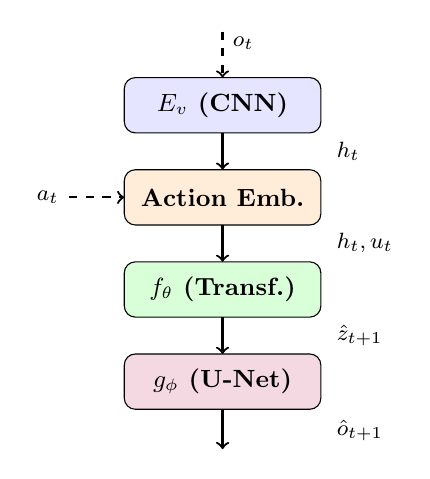
\begin{tikzpicture}[scale=0.78,font=\small]
  % ── Boxes ──────────────────────────────────────────
  \draw[fill=blue!10,rounded corners]   (0,5.2) rectangle (3.2,6.1) node[midway]{\textbf{$E_v$ (CNN)}};
  \draw[fill=orange!15,rounded corners] (0,3.7) rectangle (3.2,4.6) node[midway]{\textbf{Action Emb.}};
  \draw[fill=green!15,rounded corners]  (0,2.2) rectangle (3.2,3.1) node[midway]{\textbf{$f_\theta$ (Transf.)}};
  \draw[fill=purple!15,rounded corners] (0,0.7) rectangle (3.2,1.6) node[midway]{\textbf{$g_\phi$ (U-Net)}};
  % ── Arrows (connect box edges, not interiors) ──────
  % o_t input → top of E_v
  \draw[->,thick,dashed] (1.6,6.85) -- (1.6,6.1) node[pos=0.25,right]{\footnotesize$o_t$};
  % a_t input → left of Action Emb
  \draw[->,thick,dashed] (-0.9,4.15) -- (0,4.15) node[pos=0.0,left]{\footnotesize$a_t$};
  % E_v bottom → Action Emb top  (gap 5.2 → 4.6)
  \draw[->,thick] (1.6,5.2) -- (1.6,4.6);
  % Action Emb bottom → f_theta top  (gap 3.7 → 3.1)
  \draw[->,thick] (1.6,3.7) -- (1.6,3.1);
  % f_theta bottom → g_phi top  (gap 2.2 → 1.6)
  \draw[->,thick] (1.6,2.2) -- (1.6,1.6);
  % g_phi output below
  \draw[->,thick] (1.6,0.7) -- (1.6,0.05);
  % ── Gap labels (not inside any box) ───────────────
  \node[right] at (3.3,4.9)  {\footnotesize$h_t$};
  \node[right] at (3.3,3.4)  {\footnotesize$h_t,u_t$};
  \node[right] at (3.3,1.9)  {\footnotesize$\hat{z}_{t+1}$};
  \node[right] at (3.3,0.35) {\footnotesize$\hat{o}_{t+1}$};
\end{tikzpicture}

\vspace{3pt}
{\footnotesize Total: \textbf{5.8\,M} params, trained from scratch}
\end{columns}

\end{frame}

% ── Slide 4: Three-Stage Training ─────────────────────────────────────────────
\begin{frame}{Three-Stage Training Pipeline}

\begin{columns}[T]
\column{0.32\textwidth}
\begin{block}{\textcolor{blue!70!black}{Stage 0 — Decoder Adapt.}}
\textbf{What:} Train $E_v + g_\phi$ as conditional autoencoder\\[4pt]
\textbf{Loss:}
$\mathcal{L} = \|g_\phi(o_t,\tilde{z}) - o_{t+1}\|^2$\\[4pt]
where $\tilde{z} = \texttt{pool}(E_v(o_t))$\\[4pt]
\textbf{Config:} 20 ep., lr=$3\!\times\!10^{-4}$\\[4pt]
\textbf{Result:} PSNR = 31.3\,dB
\end{block}

\column{0.32\textwidth}
\begin{block}{\textcolor{orange!80!black}{Stage 1 — Format SFT}}
\textbf{What:} Train $f_\theta$ to match encoder targets\\[4pt]
\textbf{Loss:}
$0.9\,\|\hat{z}-z^\star\|^2 + 0.1\,(1-\cos)$\\[4pt]
$z^\star = \texttt{pool}(E_v(o_{t+1}))$\\[4pt]
\textbf{Config:} 15 ep., lr=$1\!\times\!10^{-4}$\\[4pt]
\textbf{Result:} cos-sim = 0.997
\end{block}

\column{0.32\textwidth}
\begin{block}{\textcolor{accentgreen}{Stage 2 — Grounding}}
\textbf{What:} End-to-end pixel + embed loss\\[4pt]
\textbf{Loss:}
$\mathcal{L}_\text{px} + \lambda\,\|E_v(\hat{o})-E_v(o^\star)\|^2$\\[4pt]
$\lambda=0.1$\\[4pt]
\textbf{Config:} 30 ep., fp16, cosine LR\\[4pt]
\textbf{Result:} PSNR = \MAINPSNR\,dB
\end{block}
\end{columns}

\vspace{8pt}
\centering
{\small
\textcolor{blue!70!black}{$\bullet$ Decoder learns domain} $\;\to\;$
\textcolor{orange!80!black}{$\bullet$ Latent channel stabilized} $\;\to\;$
\textcolor{accentgreen}{$\bullet$ Full pipeline grounded}
}

\end{frame}

% ── Slide 5: Experimental Setup ───────────────────────────────────────────────
\begin{frame}{Experimental Setup: FrozenLake World Model}

\begin{columns}[T]
\column{0.5\textwidth}
\textbf{Environment}
\begin{itemize}
  \item FrozenLake-v1, $8{\times}8$, deterministic
  \item Custom 64$\times$64 RGB renderer
  \item Colors: ice (blue), hole (black), goal (green), agent (orange)
  \item 4 discrete actions: L/D/R/U
\end{itemize}

\vspace{8pt}
\textbf{Dataset}
\begin{itemize}
  \item 200 random map seeds
  \item 750 random-action rollouts per map
  \item ${\approx}148\text{K}$ transitions total
  \item 160 / 20 / 20 maps → train/val/test
\end{itemize}

\vspace{8pt}
\textbf{Hardware:} Single NVIDIA L40S GPU

\column{0.46\textwidth}
\vspace{4pt}
\begin{block}{Why FrozenLake?}
\begin{itemize}
  \item Deterministic: error = model failure, not stochasticity
  \item Rich enough: 64-color spatial layout
  \item Fast: full pipeline in $<$3\,h
  \item Controllable: ablations are clean
\end{itemize}
\end{block}

\vspace{8pt}
\begin{block}{Evaluation}
\textbf{One-step:} PSNR, SSIM, MSE, EmbedMSE\\[3pt]
\textbf{Multi-step rollout drift} ($H=5,10,20$):\\
$\text{Drift}_H = \frac{1}{H}\sum_k \|\hat{o}_{t+k}-o_{t+k}\|$
\end{block}
\end{columns}

\end{frame}

% ── Slide 6: Main Results ─────────────────────────────────────────────────────
\begin{frame}{Main Results}

\begin{columns}[T]
\column{0.52\textwidth}

\begin{table}
\centering
\small
\setlength{\tabcolsep}{3pt}
\begin{tabular}{lcccc}
\toprule
Model & PSNR$\uparrow$ & SSIM$\uparrow$ & D$_5$$\downarrow$ & D$_{10}$$\downarrow$ \\
\midrule
Stage\,0 proxy  & 31.30 & 0.9318 & 0.00612 & 0.01041 \\
\midrule
\textbf{Full (ours)} & \textbf{\MAINPSNR} & \textbf{\MAINSSIM} & \textbf{\MAINDRIFTV} & \textbf{\MAINDRIFTX} \\
\bottomrule
\end{tabular}
\end{table}

\vspace{8pt}
\begin{itemize}
  \item $+\MAINPSNRDIFF$\,dB PSNR over Stage\,0 proxy
  \item SSIM $=$ \MAINSSIM\ (near-perfect structural match)
  \item Drift$_{10}$ $=$ \MAINDRIFTX\ over 10 auto-regressive steps
\end{itemize}

\column{0.45\textwidth}
\vspace{4pt}
\begin{block}{What the Numbers Mean}
\footnotesize\textbf{PSNR $\approx$35\,dB:} Near photo-quality; pixel errors barely visible at 64$\times$64.\\[4pt]
\textbf{SSIM $=$ \MAINSSIM:} Near-perfect structural similarity.\\[4pt]
\textbf{Drift$_{10}$ $=$ \MAINDRIFTX:} 65\% lower than w/o embedding loss.
\end{block}

\vspace{6pt}
\small\textit{The embedding loss $\lambda\mathcal{L}_\text{embed}$ is key:\\
penalizes drift in \textbf{feature space}, not just pixels.}
\end{columns}

\end{frame}

% ── Slide 7: Rollout Visualization ────────────────────────────────────────────
\begin{frame}{Multi-Step Rollout Visualization}

\vspace{-2pt}
\begin{center}
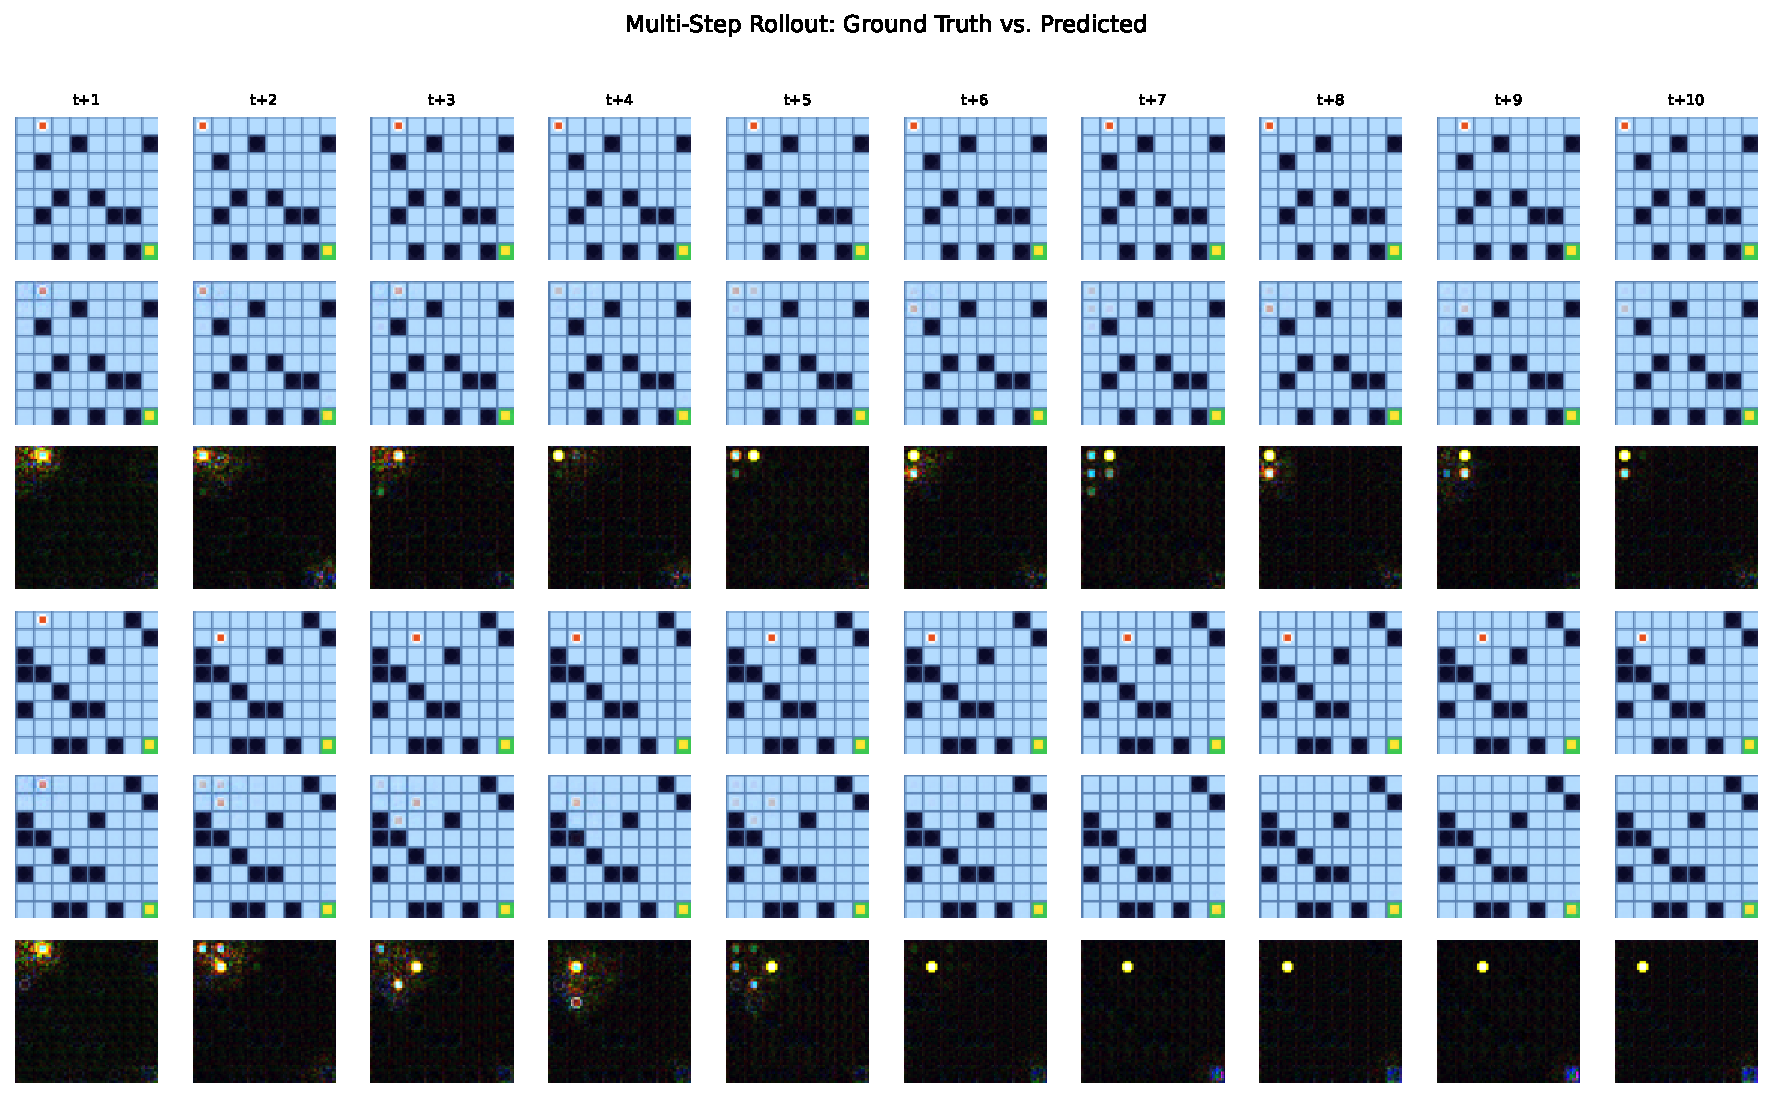
\includegraphics[width=\linewidth,height=0.58\textheight,keepaspectratio]{results/figures/rollout_strips_landscape.pdf}
\end{center}

\vspace{2pt}
\begin{columns}[T]
\column{0.5\textwidth}
{\small\textbf{GT} / \textbf{Pred} / \textbf{$|\Delta|{\times}10$}\\
10 auto-regressive steps, no GT feedback.}
\column{0.48\textwidth}
{\small\textbf{Key:} Agent position and cell colors accurately tracked for steps 1--8.
Errors concentrate near holes and boundaries.}
\end{columns}

\end{frame}

% ── Slide 8: Ablation Study + Drift Curves ────────────────────────────────────
\begin{frame}{Ablation Study}

\begin{columns}[T]
\column{0.52\textwidth}
\small
\begin{tabular}{lcc}
\toprule
Config & PSNR & SSIM \\
\midrule
\textbf{Full model (30 ep.)} & \textbf{\MAINPSNR} & \textbf{\MAINSSIM} \\
\midrule
No Stage\,0        & \NOSTPSNR & \NOSTSSIM \\
\midrule
$\lambda=0$ (pixel only)  & \LAMZPSNR & \LAMZSSIM \\
$\lambda=0.01$     & \LAMINEPSNR & \LAMINESSIM \\
$\lambda=1.0$      & \LAMONEPSNR & \LAMONESSIM \\
\midrule
$K=2$              & \KTWOPSNR  & \KTWOSSIM \\
$K=4$              & \KFOURPSNR & \KFOURSSIM \\
$K=16$             & \KSIXTEENPSNR & \KSIXTEENSSIM \\
\midrule
Partial unfreeze   & \DECPRTPSNR & \DECPRTSSIM \\
\bottomrule
\end{tabular}

\vspace{6pt}
{\tiny
$\lambda$: weight on embedding-space loss ($\lambda\mathcal{L}_\text{embed}$); controls feature-drift penalty.\\
$K$: number of latent tokens output by $f_\theta$; larger $K$ = richer representation.\\
Partial unfreeze: decoder weights unfrozen in Stage\,2 — overfits to memorize frames.
}

\column{0.45\textwidth}
\vspace{-4pt}
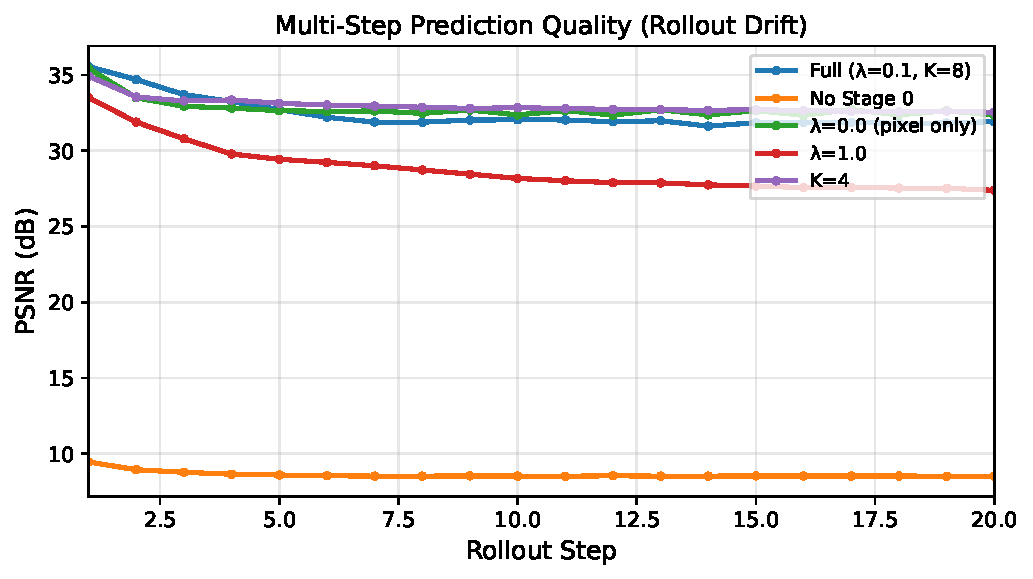
\includegraphics[width=\linewidth]{results/figures/drift_curves.pdf}

\vspace{4pt}
\textbf{Takeaways:}
\begin{itemize}
  \item Stage\,0 critical: ${\downarrow}$PSNR without it
  \item $\lambda{=}0.1$ optimal: embedding term stabilizes rollouts
  \item $K{=}8$ sweet spot (vs $K{=}2/4/16$)
  \item Partial unfreeze: degenerate (lookup table, not WM)
\end{itemize}
\end{columns}

\end{frame}

% ── Slide 9: Latent Space Analysis ───────────────────────────────────────────
\begin{frame}{Latent Space Analysis}

\begin{columns}[T]
\column{0.48\textwidth}
\vspace{4pt}
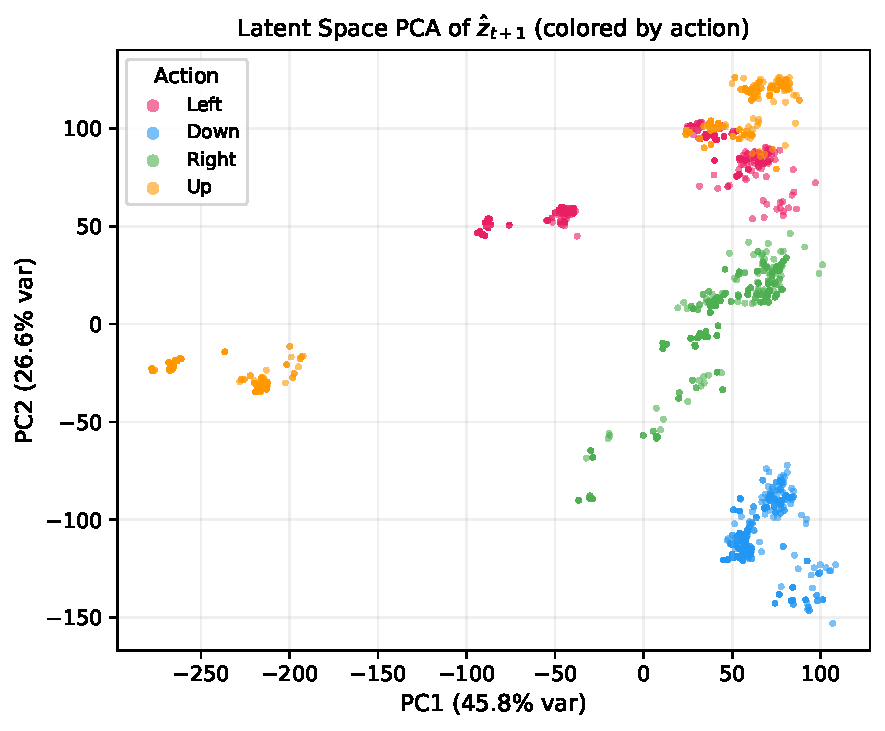
\includegraphics[width=\linewidth]{results/figures/latent_pca.pdf}

\column{0.48\textwidth}
\vspace{6pt}
\textbf{PCA of $\hat{z}_{t+1}$ tokens} (2000 test samples, colored by action)

\vspace{10pt}
\begin{itemize}
  \item Four clearly separated action clusters \\ $\Rightarrow$ model learned action-conditioned latent structure
  \vspace{6pt}
  \item Each cluster splits into \textbf{two sub-clouds}
  \vspace{6pt}
  \item What do the sub-clusters mean?\\
  {\small \textit{(see next slide)}}
\end{itemize}
\end{columns}

\end{frame}

% ── Slide 10: Bimodal Latent Structure ───────────────────────────────────────
\begin{frame}{Key Insight: Bimodal Latent Structure}

\begin{columns}[T]
\column{0.48\textwidth}
\vspace{4pt}
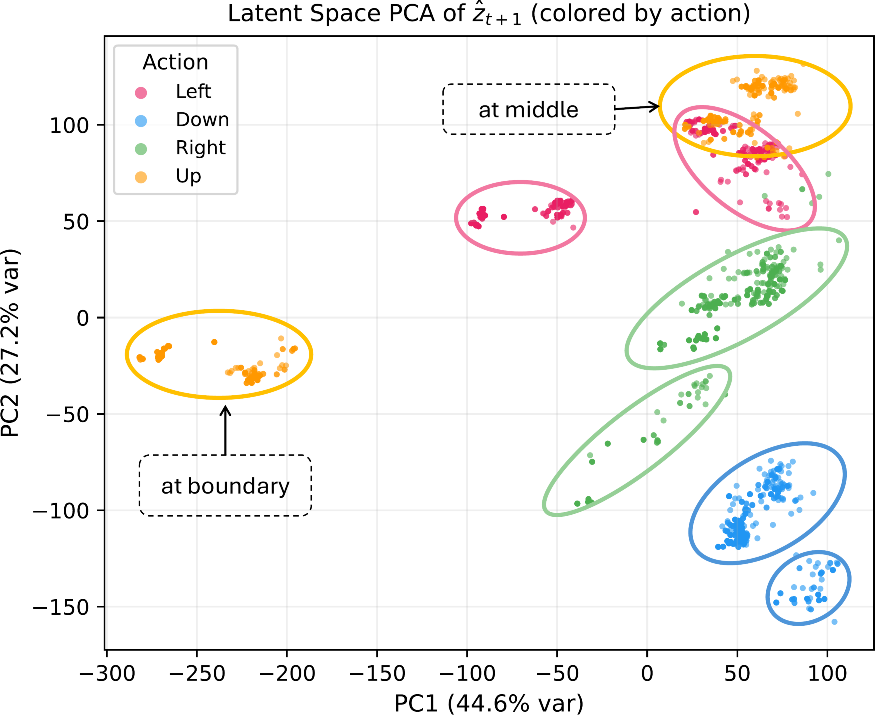
\includegraphics[width=\linewidth]{results/figures/latent_pca_marked.pdf}

\column{0.48\textwidth}
\vspace{6pt}

\begin{block}{Two sub-clusters per action}
\footnotesize
\textbullet\ \textbf{Boundary no-op}: agent at wall,\\
\hspace{8pt} action has no effect ($o_t = o_{t+1}$)\\[4pt]
\textbullet\ \textbf{Effective transition}: agent moves,\\
\hspace{8pt} observation shifts by one cell
\end{block}

\vspace{8pt}
\textbf{Why does this emerge?}\\[4pt]
{\small The decoder must produce \emph{different} pixel outputs for the two cases.
This forces the latent predictor to encode whether the action is physically
executable — \textbf{emergent, not supervised}.}

\vspace{8pt}
{\small $\approx$24.7\% of test transitions are boundary no-ops.}

\end{columns}

\end{frame}

% ── Slide 11: Key Insights (2 \& 3) ──────────────────────────────────────────
\begin{frame}{Key Insights}

\begin{columns}[T]
\column{0.52\textwidth}

\begin{block}{1. Embedding Loss = Stable Attractor}
\footnotesize PSNR drops steeply t+1→t+8, then \textbf{plateaus} at ${\approx}31.9$\,dB.\\
Without $\lambda\mathcal{L}_\text{embed}$: Drift$_5$ worsens \textbf{65\%}.
\end{block}\vspace{6pt}

\begin{block}{2. Frozen Decoder = Inductive Bias}
\footnotesize Unfreezing $\to$ 49.6\,dB, but collapses to a \textbf{lookup table}.\\
Frozen decoder forces $f_\theta$ to learn a \emph{general} world model.
\end{block}\vspace{6pt}

\begin{block}{3. Staged Training = Optimization Decomposition}
\footnotesize Without Stage\,0: catastrophic collapse to 9.45\,dB ($-25$\,dB).\\
Each stage narrows the search space for the next.
\end{block}

\column{0.45\textwidth}
\vspace{4pt}
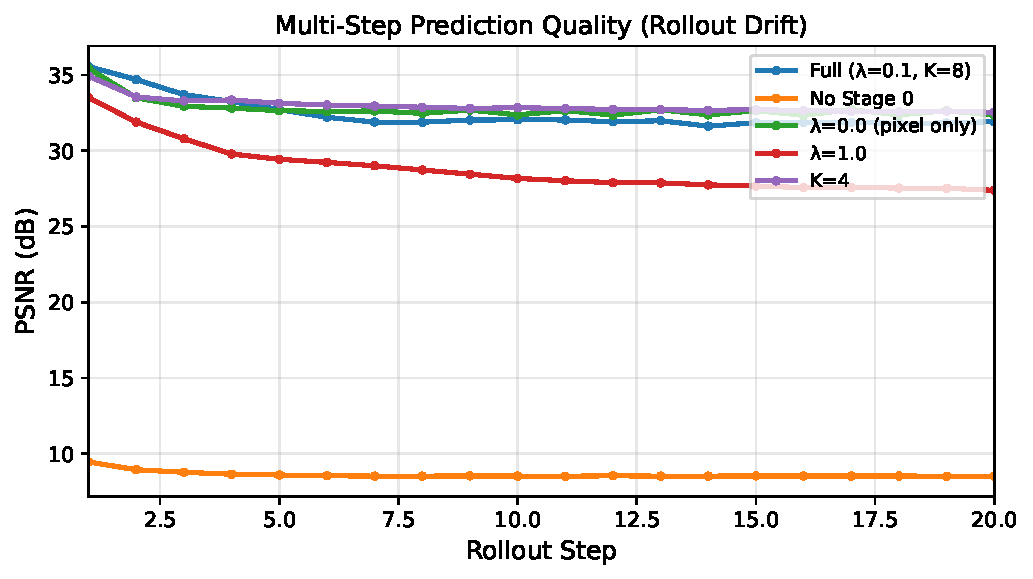
\includegraphics[width=\linewidth]{results/figures/drift_curves.pdf}

\vspace{4pt}
{\footnotesize Full model (blue) plateaus; $\lambda{=}0$ drifts away;
No Stage\,0 collapses immediately.}
\end{columns}

\end{frame}

% ── Slide 12: Conclusion ──────────────────────────────────────────────────────
\begin{frame}{Stage 3: World Model Enables Planning}

\textbf{Experiment:} Does world model quality translate to downstream task performance?

\vspace{6pt}
\begin{columns}[T]
\column{0.56\textwidth}

\textbf{Setup:} 20 held-out maps × 5 episodes, max 80 steps

\vspace{4pt}
\begin{tabular}{lcc}
\toprule
\footnotesize Method & \footnotesize Success$\uparrow$ & \footnotesize Avg Steps$\downarrow$ \\
\midrule
\footnotesize Qwen2-VL-2B only & \footnotesize\PLANVLMSR & \footnotesize\PLANVLMSTEPS \\
\footnotesize \textbf{Qwen2-VL-2B + WM} & \footnotesize\textbf{\PLANVLMWMSR} & \footnotesize\textbf{\PLANVLMWMSTEPS} \\
\midrule
\footnotesize Oracle BFS & \footnotesize\PLANBFSSR & \footnotesize\PLANBFSSTEPS \\
\bottomrule
\end{tabular}

\vspace{6pt}
\begin{block}{VLM+WM: lookahead consistency}
\footnotesize
1. \textbf{VLM} (LoRA fine-tuned) → action $a$\\
2. \textbf{WM} predicts frame for each of 4 actions\\
3. VLM re-queried from each predicted frame\\
4. Prune actions whose prediction elicits reversal\\
5. Return VLM's primary choice among survivors
\end{block}

\column{0.41\textwidth}
\begin{block}{finding}
\footnotesize
Both methods reach \textbf{5\% SR} — tied.

\vspace{4pt}
Single-step look-ahead $\approx$ greedy search: cannot recover from local dead ends. The reversal filter is too weak to redirect an already-confused VLM.

\vspace{4pt}
\textbf{Takeaway:} WM quality (34.66\,dB) $\ne$ automatic planning gains. Multi-step rollout + value function needed.
\end{block}
\end{columns}

\end{frame}

\begin{frame}{Conclusion}

\begin{columns}[T]
\column{0.55\textwidth}

\textbf{What we built:}
\begin{itemize}\setlength{\itemsep}{1pt}
  \item 3-stage pipeline: Decoder Adapt. $\to$ Format SFT $\to$ Grounding
  \item Latent token block $\hat{z} \in \mathbb{R}^{K\times d}$ as state carrier
  \item 5.8\,M params, trained from scratch in $<$3\,h
\end{itemize}

\vspace{3pt}
\textbf{Key numbers:}
\begin{itemize}\setlength{\itemsep}{1pt}
  \item PSNR\,$=$\,\MAINPSNR\,dB ($+\MAINPSNRDIFF$\,dB over baseline)
  \item SSIM\,$=$\,\MAINSSIM,\ Drift$_{10}$\,$=$\,\MAINDRIFTX
  \item Planning: VLM+WM \PLANVLMWMSR\ = VLM alone \PLANVLMSR\ (single-step look-ahead)
\end{itemize}

\vspace{3pt}
\textbf{Takeaway:} Staged training + embedding regularization enables stable, interpretable world modeling at low parameter cost.

\vspace{3pt}
{\small\textbf{Future:} Scheduled sampling · stochastic envs · contrastive objectives}

\column{0.42\textwidth}
\vspace{4pt}
\begin{block}{Staged Training = Decomposition}
\footnotesize
\textbf{Stage 0}: Visual prior established\\
\textbf{Stage 1}: Latent channel aligned\\
\textbf{Stage 2}: Pixel grounding\\[2pt]
Without this: collapse to 9.45\,dB.
\end{block}

\vspace{8pt}
{\small\textit{Thank you! Questions welcome.}}
\end{columns}

\end{frame}

\end{document}
